\documentclass[12pt]{article}

\usepackage{graphicx}
%\usepackage{apacite}

\title{Analysis of a Professional Journal Article}
\author{
        Partha Sarathi Ghosh\\
        Computer Engineering Department\\
        San Jose State University\\
        1 Washington Sq, San Jose, CA 95192 \underline{USA}
}

\date{\today}

\begin{document}
\maketitle
\pagenumbering{roman}
\pagebreak

%\begin{abstract}
%This is the paper's abstract \ldots
%\end{abstract}

\begin{center}
\tableofcontents
\end{center}
\pagebreak
\begin{center}
\listoffigures
\end{center}
\pagebreak

\pagenumbering{arabic}

\section{Introduction}
\indent The objective of this assignment is to select a high quality technical article and review its technical content. The technical paper also needs to be critiqued based on the relevance of the content, results of the findings and address unanswered questions in the paper. \\
%The key attributes of a quality technical article are, the article should be published in only in a single journal, always peer reviewed and author need not make any payment to get the article published. In the area of computer science, American Computing Machinery (ACM) and Institute of Electrical and Electronics Engineers (IEEE) are two professional organizations, well known for publishing quality and peer reviewed technical articles. \\
This report is organized as follows. In the next section the technical paper's title and the authors \ref{ref:paper_title} are introduced, followed by the technical analysis [Section~\ref{ref:paper_discussion}] of the paper. The technical analysis section covers the motivation [Section~\ref{ref:paper_motivation}] of the paper, the problem [Section ~\ref{ref:paper_problem}] that is being solved, the methods and techniques [Section ~\ref{ref:paper_method}] the authors has used for their research, and the scope of future work [Section ~\ref{ref:paper_scope}] is. This section ends with the description of the authors' conclusion [Section ~\ref{ref:paper_conclusions}] about their research. \\
In the following section [Section ~\ref{ref:critique_discussion}], I critique the content of this paper, check the relevance of the content with respect to the title of the paper [Section ~\ref{ref:critique_motivation}], review the findings of the paper [Section ~\ref{ref:critique_problem}], highlight any unanswered questions [Section ~\ref{ref:critique_method}] by the authors. I also review the literature style of the technical paper [Section ~\ref{ref:critique_scope}] from writing style and visual aid used. The conclusion [Section~\ref{ref:critique_conclusions}] of this report highlight my concluding remarks on this literature review assignment.
% \indent I'm pursuing a Masters in Software Engineering and my specialization is in Cyber Security.
\section{Title of the Technical Paper} \label{ref:paper_title}
The technical paper I selected is titled \textit{The Evolution of Android Malware and Analysis Technique} ~\cite{Tam:2017:EAM:3022634.3017427} has been published by ACM Computing Surveys (CSUR), Volume 49 Issue 4, February 2017 Article No. 76.  The technical article has been refereed, cited by 18 papers and downloaded 2832 times as of \date{November 18, 2019}. These facts about the paper indicates that this is a quality technical paper.\\

\subsection{Authors}
The authors of this paper are researchers from University of London and University of Malaya. The authors are:
\begin {itemize}
    \item Kimberly Tam, Information Security Group, Royal Holloway, University of London,
    \item Ali Feizollah, Nor Badrul Anuar, and Rosli Salleh, Department of Computer, System and Technology, University of Malaya,
    \item Lorenzo Cavallaro, Information Security Group, Royal Holloway, University of London.
\end{itemize}

\section{Technical Analysis of the Paper}\label{ref:paper_discussion}
\subsection{Summary of the Paper}
The authors describe proliferation of Android mobile devices in our lives and how it has become ubiquitous over a span of a decade. The author uses statistics from the year 2010 to 2015 to establish this facts by comparing Android usage with the other mobile operating systems. The authors establish the context for the motivation of this technical paper. Rapid proliferation of the Android mobile devices gave rise to malware at a high rate in the android mobile devices. The authors create the scope of their research \textit {"Unlike previous works, this article is not a general study on mobile \ldots but instead focuses on Android-related analysis techniques systematically and in detail"}~\cite{Tam:2017:EAM:3022634.3017427}. \\
The article walks the path of the evolution of Android malware and creates an analogy with the malware found in the early days of the personal computers(PC). However, the techniques used to develop the malware for PC is different from that of the Mobile devices. This is because of the inherent hardware architectural differences between these two computing devices. The technical paper points out the threat landscape in the domain of mobile devices, by describing the financial motivation of a malware programmer. The technical paper mention, that a malware programmer can earn up to \$12,000 a month by creating a malware. Once the android mobile device is infected with the malware, it sends out short message service (SMS) with the user's data and without the user's knowledge. Malware could also send out personal data using TCP/IP communication at wee hours when the user might be sleeping or may not have access to the Android device.\\
This paper writes in detail about the different methods of malware detection used. The authors describe the static and dynamic analysis methods and then explains how a hybrid approach could be more beneficial for malware detection. The authors say that machine learning methods, coupled with hybrid mechanism is the possible solution for malware detection in the current Android OS landscape.

\subsection{Motivation}\label{ref:paper_motivation}
The motivation of the authors is to study the current techniques used in detecting malware in Android operating system. Malware tries to take advantage of the security holes that are present in the Android operating system. If a malware gets detected by one of the sophisticated mechanism (static analysis and dynamic analysis), as described in the technical paper, the malware (creators) resort to new ways of detection evasion. One other motivation of this technical paper is to study the evasion techniques used by the malware and how its proliferation could be mitigated. Since the evolution of Android operating system has been organic between 2007-2015, the evasion of malware and detection of malware techniques are always running a race to beat each other. This has created a challenge for the researchers in the area of Android security. The author of this technical paper hypothesize a solution, to detect malware in a continuously changing threat landscape for Android OS.

\subsection{Problem Description}\label{ref:paper_problem}
Android operating system has been evolving at a very rapid pace. There has been 23 major software releases ~\cite{Tam:2017:EAM:3022634.3017427} of the Android operating system between 2010 and 2015. The velocity of these releases has made it difficult for security engineers to try to solve the security issues in the Android operating system. Android operating systems' meteoric rise in popularity (80\% of mobile devices were running malware in 2011), has been one of the primary reason for the proliferation of the malware.\\
Android operating system is based on Linux Kernel with Java programming language being the application development frame work. The key security issue in the architecture has been the permission infrastructure provided by the Android application framework. Java byte code has its inherent security issues in Java Virtual Machine (JVM), Java class libraries and associated libraries in the Android framework.

\subsection{Methods and Apparatus Used}\label{ref:paper_method}
In the Taxonomy of Mobile Malware Analysis ~\cite{Tam:2017:EAM:3022634.3017427} section in the technical paper details the ineffectiveness of malware detection, using binary signature analysis. The malware could evade detection by rearranging the text or the data section of malware binary. This creates a challenge and opportunity to the researches to look for newer techniques for malware detection. The paper looks into different techniques used in static code analysis, dynamic code analysis and a hybrid approach with great detail. For static analysis Android permission mechanism, the intent mechanism, the binary packaging layout and usage of hardware components are well researched with technical details. \\
To explain the dynamic analysis method, the paper researches into the Application Programming Interface (API) and its interaction with the kernel, to build up the security hole context. Since dynamic analysis can expose the executable part of the source code (for malware analysis), the authors describes different inputs techniques, that could be used to create a graph to explore the different paths of code execution. Dynamic analysis needs to be done at different architectural layers (Application, kernel, device drivers, hardware interactions etc.), also using different run time environments. \\
The paper also looks into the evolution of the evasion techniques used by the malware. One of the simple techniques that the malware uses is to run the application at odd hours when the users are not using the device. The authors identify that permission infrastructure is the weak point in the Android architecture. The paper tries to pivot on this architectural issues and tries to devise different malware analysis and detection methods.

\subsection{Proposed Solutions}\label{ref:paper_sol}
The number of different mobile devices that are available complicates the problem of malware detection. It's hard to perform the analysis of the malware in all the target (available) mobile devices. The paper \textit{proposes} a hybrid approach that combines static and dynamic analysis methods with use of virtual machine (VM) to simulate the multitude of target android devices for malware detection. The VM can be simulated to operate like a real hardware with certain changes in the software. \\
The paper also detail another hybrid approach in which static and dynamic analysis methods along with machine learning (ML) could be used for analysis of the malware. This method seems to be superior because it can scale to support the huge number of different hardware  android operating system is supported on. \\ 
As alternative approaches, the paper explores other techniques of identifying malware like, using network traffic analysis, code coverage of API interfaces, monitoring system calls, creation of application dependency graphs for all the applications running, information flows among the application and operating system infrastructure, inter-process communication analysis, hardware analysis and application metadata analysis. The paper also mentions that detection of  malware, after malware analysis is \textit{classification} problem. In situations where malware cannot be identified using binary classification, then different attributes of the malware needs to be analysed, thereby translating the analysis problem, to a multiple class \textit{stochastic} problem. \\ 

\subsection{Scope of Future Work}\label{ref:paper_scope}
The paper states that the future of the Android Malware research is in pursuing the path of hybrid approach, to uses static analysis, dynamic analysis, ML and use or virtual machines to simulate target hardware. The advances in parallel computing would allow the future researchers to follow the hybrid approach of malware analysis. The authors highlight the advantages of performing code coverage analysis on the applications using the hybrid mechanism. Code coverage method can present different branches of execution, which would help in identifying the weak links in an application. Since malware have started evading detection in virtualised environment, one area of research would be to use virtualisation to detect malware.

\subsection{Conclusions}\label{ref:paper_conclusions}
The author of this technical paper mention that they studied a wide range of Android malware analysis and detection frameworks. The technical paper created the context by describing the threat landscape for mobile devices, followed by the evaluation of different malware detection techniques and solutions. The authors think that they have discussed threats and solutions for android devices, and they have been able to provide a superior solution than those available. 

\section{Critique On The Paper}\label{ref:critique_discussion}
The paper is a well researched one. It details the evolution of android malware from the year 2010 to 2015. The authors have been consistent in providing relevant data from this period to substantiate their arguments. In the introduction section of the paper, the author describes their effort in details with tabular data of previous research. 

\subsection{Writing Style}\label{ref:critique_scope}
The authors have been consistent in their style of writing throughout the 40-page article. Each section builds up of context before highlighting the problem, analysing the problem finally reaching  to a conclusion or solution. \\
The paper should have had separate sections describing the packaging mechanism in android. There should have been a separate section in it, on the android file system layout. These are key areas that opens up security holes in Android. The authors should have added these section for more clarity for the readers. \\
\subsubsection{Visual Aids}
The author substantiate their arguments with relevant statistics using numerous tables and graphs. In one of the graphs, the smart phone operating systems market share data \ref{lbl_smartphone_market_share} serves well as a visual aid for the reader.
\begin{figure}[h!]
%\begin{figure}
        \centerline{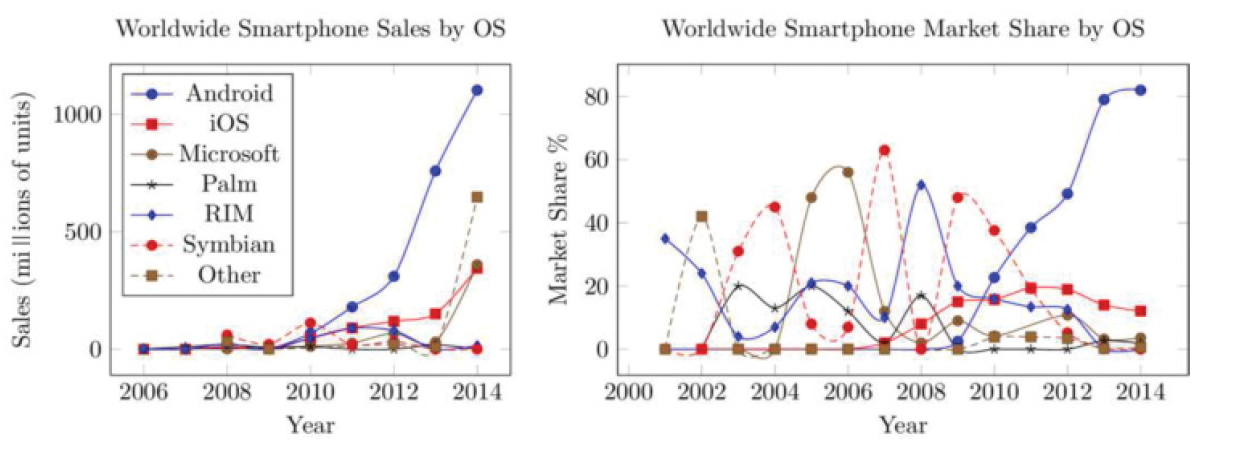
\includegraphics[scale=0.45]{smartphonemarketshare.PNG}}
        \label{lbl_smartphone_market_share}
        \caption{Smartphone market share, ~\cite[fig 1]{Tam:2017:EAM:3022634.3017427}}
\end{figure}
\begin{figure}[h!]
        \centerline{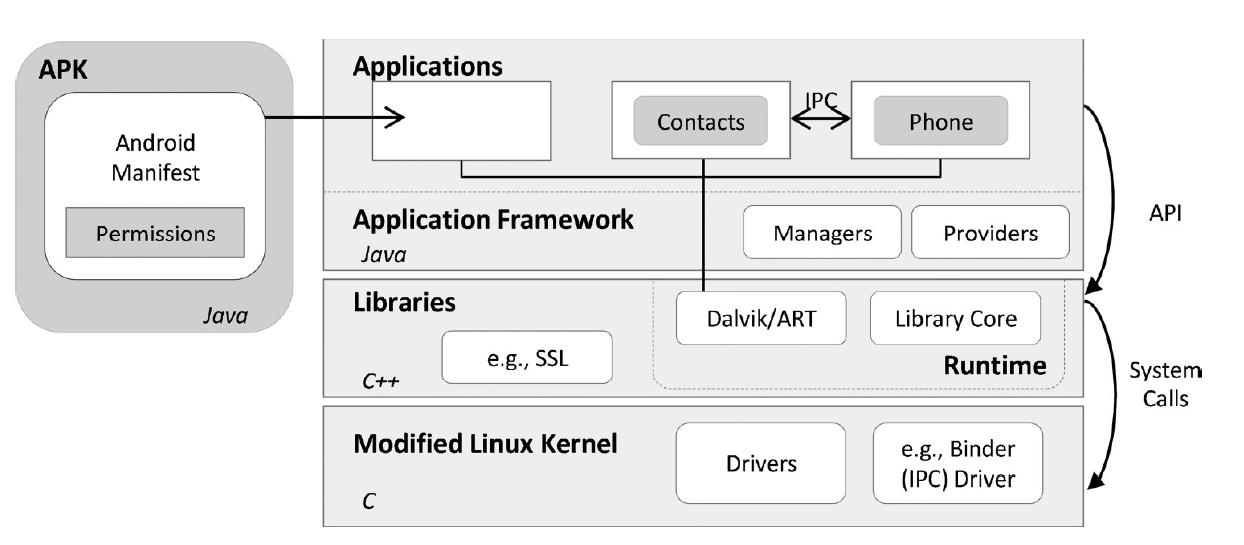
\includegraphics[scale=0.45]{androidlinuxkernel.PNG}}
        \caption{Overview of Andriod Operaing System Architecture ~\cite[fig 2]{Tam:2017:EAM:3022634.3017427}}
        \label{lbl_linux_kernl}
\end{figure}
These tables used are important tools for conveying complex data to the readers. Since the paper traverses evolution of malware with the proliferation of Android from the year 2010 to 2015, there are graphs to show progression of a single data annually, like mobile usage among people, worldwide smartphone market shares. Another good example of visual aid is the description of Android Linux kernel using a figure \ref{lbl_linux_kernl}. Any reader would appreciate the clarity of the system blocks in this architectural diagram. \\
\begin{figure}[h!]
        \centerline{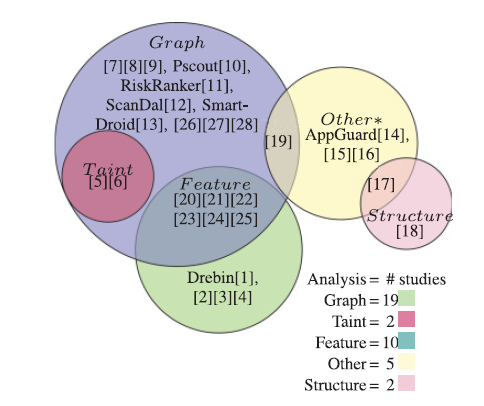
\includegraphics[scale=0.45]{venn_diagram.PNG}}
        \caption{Venn diagram of static analysis methods ~\cite[fig 3 b]{Tam:2017:EAM:3022634.3017427}}
        \label{lbl_venn}
\end{figure}
In the diagram ~\ref{lbl_venn} the authors citations overwhelms the Venn diagram. The Venn diagram tries to explain the different static analysis methods used in Android OS. The author could have used indirections to remove place the citations differently in a separate table. This Venn diagram should have had only the static analysis methods and descriptions. Thus, in this particular case the purpose of the Venn diagram is defeated. \\

\subsection{Relevance of the Content}\label{ref:critique_motivation}
The paper describes Android architecture with a few diagrams. This is important for the reader who may not be familiar with the Android architecture. It must be noted here that though Android operating system has a Linux kernel but the application architecture is different. This is because most of the mobile devices that has Android operating system uses the ARM hardware architecture, smaller power requirements, different storage hardware etc.\\ 
The usage of tables to illustrate different multi variable comparison is very apt. This helps to read the document more effectively and identify the points of differentiation with greater clarity. The paper uses graphs to demonstrate single variable changes over the years for example fig 1~\cite{Tam:2017:EAM:3022634.3017427}. The explanation of the dynamic analysis and static analysis are written with great detail. Other mobile operating system are detailed in this paper. I think this is redundant because the focus of the paper is on Android operating system, it was unnecessary to explain any of the other mobile operating systems as the security features of those devices are not in the scope of this research. The paper should have provided details on the VM, JIT and ART, as there are variants of implementation. VM, JIT and ART are integral part to devise any security mechanism in Android operating system.

\subsection{Results of the Findings}\label{ref:critique_problem}
The authors have researched extensively over 100 technical papers. To substantiate their argument the author have compared papers and those papers approach on malware detection. This technical paper is filled with references of statistics like growth percentage of malware year over year, usage of different mobile operating system, financial incentive of a malware etc. The paper also look at the types of static analysis methods and dynamic analysis methods. The paper looks into different techniques of dynamic analysis. Paper concludes with empirical evidence that a hybrid approach would be the way for the future of malware analysis and detection. The finding of the researchers are significant because the authors realize that mobile device ecosystem is dynamic and only a hybrid approach will lead to effective solution for malware detection.

\subsection{Unanswered Questions}\label{ref:critique_method}
One of the primary reason for the proliferation of the Android malware is the failure of app store to check for malicious application. The paper should have detailed the mechanism of application upload and application distribution in app store. A section should have been written about this in the technical paper. The paper do not describe the installation process of application in Android operating system. Detail on the tools that had been used for this research is missing. The paper do not rule out or talk about the flaws in ARM architectures which could be reason malware proliferation in Android.

\section{Conclusions}\label{ref:critique_conclusions}
As a graduate student this was an opportunity to review a paper for its technical content and then critique it. The process was rigorous involving multiple reading, creating notes and then assimilating the notes into a report, writing the report with multiple rounds of proof-reading. The learning from this exercise has been positive. This experience would be useful while I write my master's thesis.
%\bibliographystyle{apacite}
\bibliographystyle{abbrv}
\bibliography{reportAnalysisOfAProfessionalJournalArticle}


\end{document}
This is never printed
